\chapter{Loops and Array}
\section{Goals}
\begin{itemize}
%    \item Mahasiswa dapat mengenal dan menggunakan perulangan while pada bahsa C
    \item Students are able to use while-loop on C
    %\item Mahasiswa dapat mengenal dan menggunakan perulangan do-while pada bahasa C
    \item Students are able to use do-while loop on C
    %\item Mahasiswa dapat mengenal dan menggunakan perulangan for pada bahasa C
    \item Students are able to use for loop on C
    %\item Mahasiswa dapat mengenal dan menggunakan  array dimensi satu maupun multidimensi.
    \item Students are able to use one dimensional or multidimensional array
    %\item Mahasiswa mampu memanfaatkan perulangan untuk mengolah data pada array.
    \item Students are able to use loops to process data on arrays
\end{itemize}
\section{Loop}
\subsection{while loop}
%Perulangan while akan menjalankan blok kode yang berada di dalamnya selama kondisi perulangan masih bernilai benar.
While loop will run the code block within it repeatedly as long as the loop condition is true


\begin{figure}[H]
		\centering
		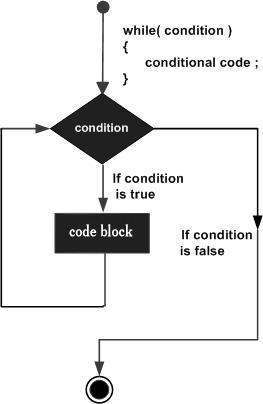
\includegraphics[width=0.4\linewidth]{PerulanganDanArray/whileloop}
		\caption{Flow chart of while loop}
		\label{fig:whileloop}
\end{figure}

%yntaxnya pada bahasa C adalah sebagai berikut:
Its syntax in C programming language is as follows
\begin{verbatim}
    while(Condition)
    {
        // The block of code that will be repeated
    }
\end{verbatim}

%Sebagai contoh, perhatikan kode berikut
As an example, look at the following code
\begin{lstlisting}[language=c,caption = Contoh Penggunaan while,label=lst:whileexample01]
int main()
{
	int uangSaya,hargaRoti;
	uangSaya = 10000;
	hargaRoti = 2000;
	while(uangSaya >= hargaRoti)
	{
	    printf("Beli roti 1, uang saya sisa %d", uangSaya - hargaRoti);
	    uangSaya -= hargaRoti;
	}
	printf("Uang saya tidak cukup lagi");
	return 0;
}
\end{lstlisting}  
The output of the program in Listing \ref{lst:whileexample01} are
\begin{verbatim}
    Beli roti 1, uang saya sisa 8000
    Beli roti 1, uang saya sisa 6000
    Beli roti 1, uang saya sisa 4000
    Beli roti 1, uang saya sisa 2000
    Beli roti 1, uang saya sisa 0
    Uang saya tidak cukup lagi
\end{verbatim}

%Pada contoh ini, operasi pada baris 9 membuat variabel \verb|uangSaya| berkurang 2000 pada setiap pengulangan hingga akhirnya nilai \verb|uangSaya| tidak lebih dari atau sama dengan \verb|hargaRoti| lagi.
You can see the line 9 of the code causes the variable \verb|uangSaya| to have its value substracted by 2000 for every loop until \verb|uangSaya| is no longer greater than equal to \verb|hargaRoti|. 
The loop condition will be invalid and finaly exits the loop. Then it prints "Uang saya tidak cukup lagi", the command after the while loop statement.
\subsection{do-while loop}
%do-while loop sebenarnya sama seperti while loop hanya saja do-while akan menjalankan perintah pada blok kode didalamnya terlebih dahulu sebelum melakukan pengecekan kondisi.
do-while loop is very similar to while loop. The only difference is that do-while loop will execute the code block inside it once, and then checks the condition.
\begin{figure}[H]
		\centering
		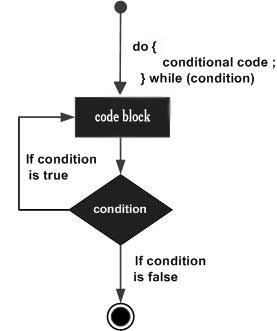
\includegraphics[width=0.4\linewidth]{PerulanganDanArray/dowhileloop}
		\caption{do-while flow chart}
		\label{fig:dowhileloop}
\end{figure}
%Syntaxnya pada bahasa C adalah sebagai berikut:
Its syntax in C is as follows:
\begin{verbatim}
    do{
        // the block of code that will be repeated
    }while(Condition)
\end{verbatim}
%Sebagai contoh, perhatikan kode berikut
Look at the following example.
\begin{lstlisting}[language=c,caption = Contoh Penggunaan do-while,label=lst:dowhileexample01]
int main()
{
	int uangSaya,hargaRoti;
	uangSaya = 10000;
	hargaRoti = 12000;
	do{
	    printf("Beli roti 1, uang saya sisa %d", uangSaya - hargaRoti);
	    uangSaya -= hargaRoti;
	}while(uangSaya >= hargaRoti)
	printf("Uang saya tidak cukup lagi");
	return 0;
}
\end{lstlisting}  
%Output dari program pada Listing \ref{lst:dowhileexample01} adalah
The output of the code above are
\begin{verbatim}
    Beli roti 1, uang saya sisa -2000
    Uang saya tidak cukup lagi
\end{verbatim}
The variable \verb|uangSaya| is substracted by \verb|hargaRoti| before checking the \verb|uangSaya>=hargaRoti| condition.
Had the code above uses while loop, the repeating block of code wouldn't have executed even once.

\subsection{for loop}
%Misalkan terdapat blok kode while dengan bentuk seperti ini:
If you have a block of code like this:
\begin{verbatim}
    InitializationStatement; // e.g.: int i = 0;
    while(Condition){
        // do something
        updateStatement; // e.g.: i++ 
    }
\end{verbatim}
This is equivalent to
\begin{verbatim}
    for(InitializationStatement;Condition;updateStatement){
        // do something
    }
\end{verbatim}

%Sebagai contoh, perhatikan program berikut:
As example, look at the following code:
\begin{lstlisting}[language=c,caption = Contoh Penggunaan for,label=lst:forexample01]
int main()
{
    int i=0;
    for(i=1;i<10;i++){
        printf("%d ",i);
    }
	return 0;
}
\end{lstlisting}
%Output dari program ini adalah
The output of this program are
\begin{verbatim}
    1 2 3 4 5 6 7 8 9 
\end{verbatim}
%Berikut kode pada Listing \ref{lst:forexample01} jika diubah menjadi bentuk while-loop
The following is the code if code in Listing \ref{lst:forexample01} converted to its while-loop form
\begin{lstlisting}[language=c,caption = For dalam bentuk while,label=lst:forwhileform01]
int main()
{
    int i=0;
    i=1;
    while(i<10){
        printf("%d ",i);
        i++;
    }
	return 0;
}
\end{lstlisting}

\section{Array}
%Array atau biasa disebut larik adalah koleksi data dimana setiap elemen mempunyai nama yang sama dan bertipe sama. Setiap elemen diakses berdasarkan  indeks elemennya.
Array is a collection of data where each element of it has the same name(indexed) and data type. Every element in an array can be accessed using its element index.
\subsection{Array 1D}
%Variabel array dimensi satu dideklarasikan dengan menentukan jenis elemen dan jumlah elemen yang di perlukan oleh array. 
One dimensional array variable can be declared by deciding the data type of the element and the number of element that is needed.

Syntax:
\begin{verbatim}
    DataType variableName [arraySize];
\end{verbatim}
\begin{enumerate}
	\item \verb*|DataType|.\\
    The data type of the elements in the array, e.g. \verb|float|, \verb|int|, etc.
	%Jenis elemen data elemen array :\verb*|float|,\verb*|int|,\verb*|char| dsb
	\item \verb*|variableName|\\
	%Namariabel mengikuti aturan pemberian nama variabel,
    variableName follows the variable naming convention
	
	\item \verb*|arraySize| \\
    Integer more than 0. Defining the number of element an array has.
	%konstanta integer lebih besar dari 0. \\
\end{enumerate}

%Untuk menginisialisasi array dimensi satu, dapat dilakukan dengan cara seperti berikut:
Initializing one dimensional array can be done like shown below:
\begin{verbatim}
    int contoh_array[5] = {4,2,0,6,9};
\end{verbatim}

%Data di dalam array dapat akses dengan menggunakan suatu bilangan yang merupakan index dari array tersebut. Perhatikan potongan kode berikut.
Data in an array can be accessed by using an integer that is the index of the array. Look at the code below

\begin{lstlisting}[language=c,caption = Contoh Mengakses Array 1D,label=lst:array1d01]
int main()
{
    int arr[5] = {4,2,0,6,9};
    printf("%d\n",arr[0]);
    printf("%d\n",arr[4]);
    int i = 0;
    printf("%d\n",arr[i]);
    for(i=0;i<5;i++)
        printf("%d",arr[i]);
}
\end{lstlisting}

%Potongan kode pada Listing \ref{lst:array1d01} akan memberikan output
The code in Listing \ref{lst:array1d01} will give output
\begin{verbatim}
    4
    9
    4
    42069
\end{verbatim}

\subsection{2D Array and Other Multidimensional Arrays}%Array 2D dan Array Multidimensi lainnya}
%Array dimensi dua pada dasarnya hanya merupakan array dimensi satu dari array dimensi satu. Oleh karena itu, untuk mendeklarasikan array dimensi dua kita dapat menggunakan syntax seperti berikut.
2D array is basically a 1D array of 1D array. Intuitively, you can define a 2D array like as seen below:
\begin{verbatim}
	DataType variableName[arraySize1][arraySize2];
\end{verbatim}
%Hal ini berlaku juga untuk array dengan dimensi lebih dari dua.
This also applies to multidimensional array.
\begin{verbatim}
    DataType variableName[arraySize1]...[arraySizeN];
\end{verbatim}
There will be $arraySize_1\times arraySize_2 \times \cdots \times arraySize_n$ of elements that would be allocated to the memory after doing multidimensional array like that.

%Untuk menginisialisasi suatu array multidimensi dapat dilakukan sama seperti array biasa:
To initialize multidimensional array, you can do the following:
\begin{verbatim}
    int arr[2][2] = {{1,2},{3,4}};
\end{verbatim}

\section{Example of Using Loops and Array}
\subsection{Linear Search}
%Linear Search adalah teknik untuk mencari suatu elemen dengan mengunjungi secara berurutan tiap - tiap elemen. Berikut adalah contoh mencari bilangan terbesar pada suatu array dengan menggunakan linear search
Linear Search is a technique to search for an element by visiting each element one by one. 
The following code is an example of how to find the largest number in an array using linear search.
\begin{lstlisting}[language=c,caption = Finding the largest integer,label=lst:linearsearch01]
int main()
{
    int arr[5] = {4,2,0,6,9};
    int currentMax = arr[0];
    int i;
    for(i=0;i<5;i++){
        if(currentMax < arr[i]){
            currentMax = arr[i];
        }
    }
    printf("Bilangan terbesar adalah %d",currentMax);
}
\end{lstlisting}
\subsection{Bubble Sort}
%Bubble Sort adalah suatu algoritma untuk mengurutkan data. Berikut adalah implementasinya pada bahasa C.
Bubble Sort is a simple algorithm to sort data. The bubble sort algorithm can be seen below:
\begin{lstlisting}[language=c,caption = Bubble Sort,label=lst:bubblesort01]
int main()
{
    int arr[5] = {4,2,0,6,9};
    int tmp;
    for(int i=0;i<5;i++){
        for(int j = 0; j < 5-i-1;j++){
            if(arr[j]>arr[j+1]){
                tmp = arr[j];
                arr[j] = arr[j+1];
                arr[j+1] = tmp;
            }
        }
    }
    
    for(int i=0;i<5;i++){
        printf("%d ",arr[i]);
    }
}
\end{lstlisting}
\section{Exercise}
\begin{itemize}
    %\item Cobalah inisialisasi suatu array multidimensi dengan menggunakan perulangan for.
    \item Try to initialize a multidimensional array with for loop
    %\item Buatlah suatu program untuk mengisi data pada suatu array perdasarkan input dari keyboard.
    \item create a program to fill the data of an array by keyboard input.
    %\item Apakah yang akan terjadi jika suatu array \verb|arr| diakses dengan \verb|arr[-1]|?
    \item What would happen if an array \verb|arr| is accessed with \verb|arr[-1]|?
    %\item Apakah yang akan terjadi jika suatu array \verb|arr| dengan ukuran 5 diakses dengan \verb|arr[5]|?
    \item What would happen if an array \verb|arr| with size 5 is accessed with \verb|arr[5]|?
    \item Look at the following code
    \begin{verbatim}
        for(i=0;i<10;i++){
            for(j=i;j<10;j++){
                printf("A");
            }
        }
    \end{verbatim}
    How many "A" will be printed on the screen if that block of code is executed?
    %Ada berapa banyakah huruf A yang akan muncul pada layar jika program tersebut dijalankan?
\end{itemize}
